\subsection{Sequence Diagram}

\IfFileExists{sections/BLL/LoginSeqDiagram.pdf}{
    \begin{figure}[H]
        \centering
        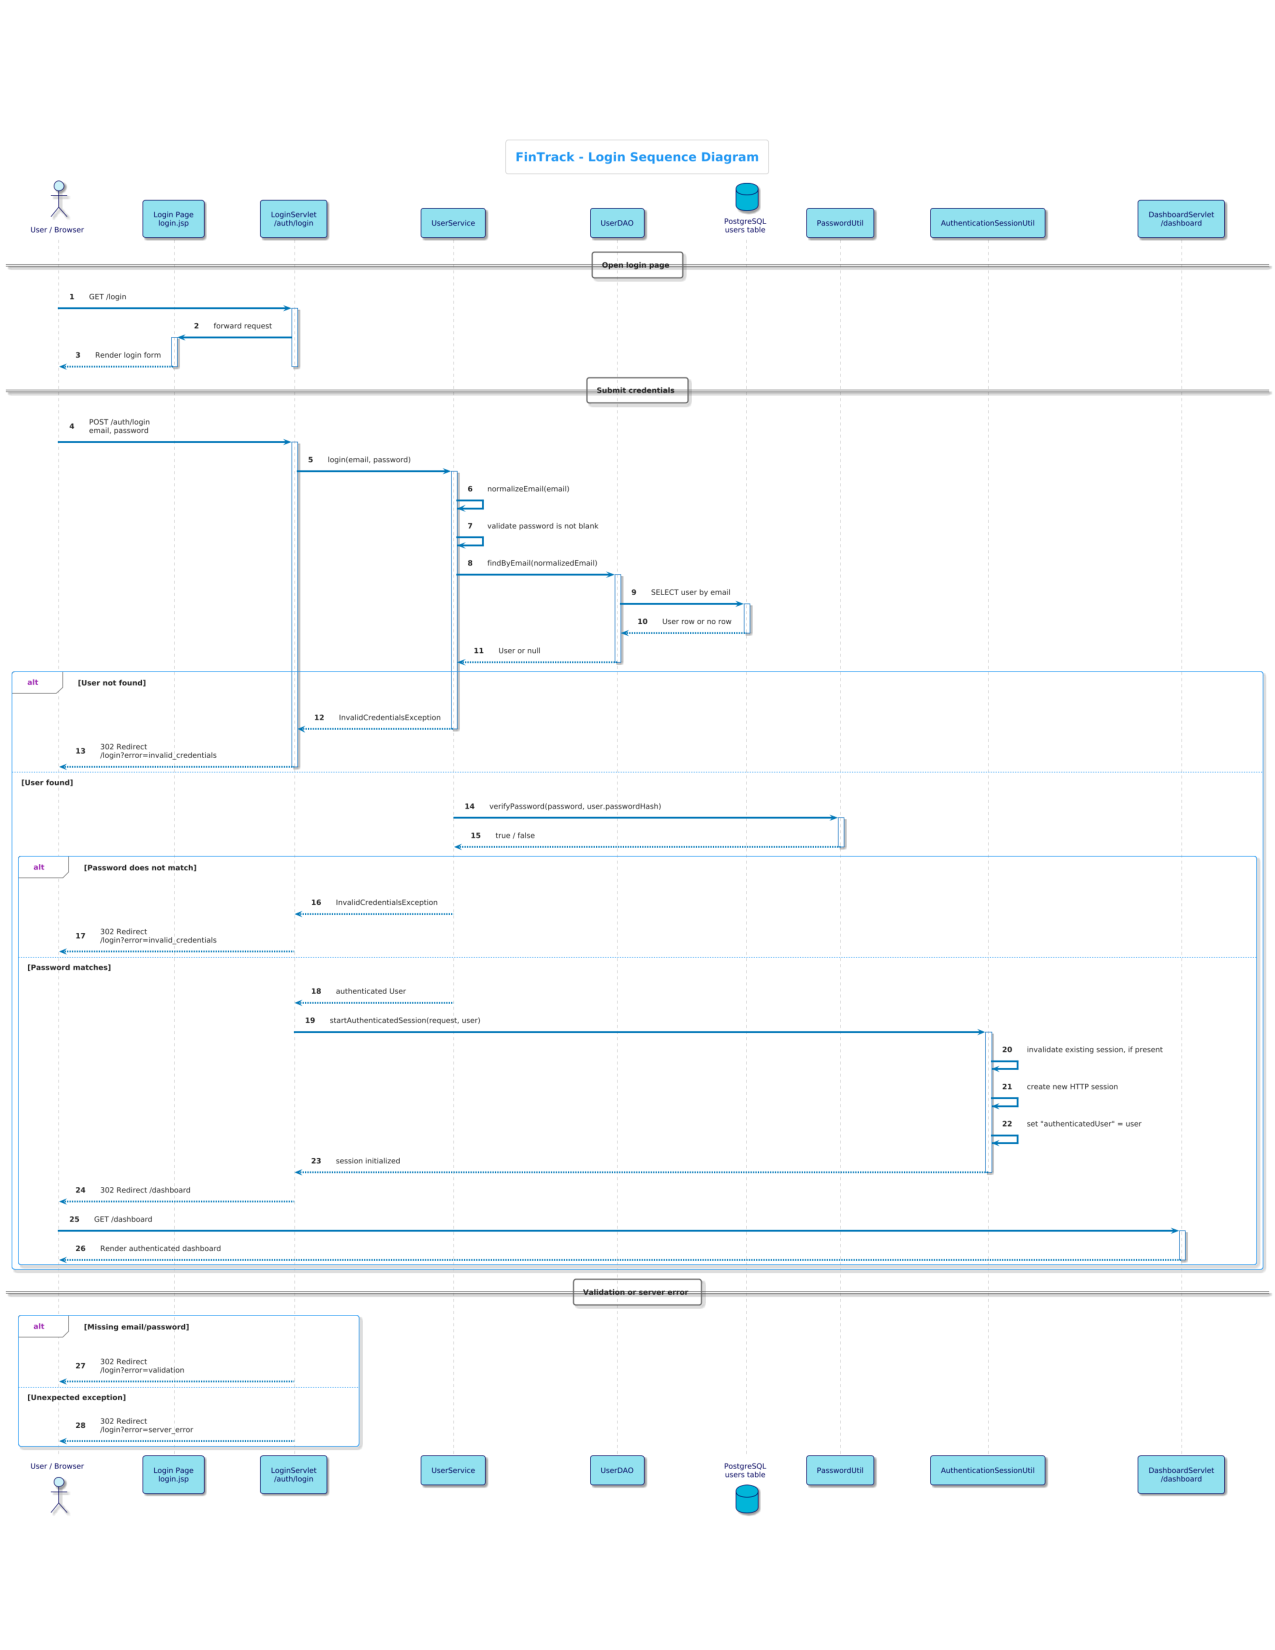
\includegraphics[width=0.95\textwidth]{sections/BLL/LoginSeqDiagram.pdf}
        \caption{Login Sequence Diagram}
    \end{figure}
}

The diagram illustrates the login flow implemented in FinTrack, from opening the login page to creating an authenticated HTTP session.
The main events are as follows:

\begin{enumerate}
    \item \textbf{Login Page Rendering:} \\
    The process starts when the browser sends a \texttt{GET /login} request.
    The request is handled by \texttt{LoginServlet}, which forwards the request to the JSP login page.
    The page renders the form where the user can enter an email address and password.

    \item \textbf{Login Request Processing:} \\
    When the form is submitted, the browser sends a \texttt{POST /auth/login} request to \texttt{LoginServlet}.
    The servlet extracts the credentials from the request and delegates the authentication logic to \texttt{UserService}.
    The service performs the core checks by:
    \begin{itemize}
        \item Normalizing the email address and validating that the password is not blank.
        \item Loading the corresponding user record through \texttt{UserDAO}.
        \item Querying the PostgreSQL \texttt{users} table for a matching email address.
        \item Verifying the submitted password against the stored hash through \texttt{PasswordUtil}.
    \end{itemize}

    \item \textbf{Outcome Handling:} \\
    The final outcome depends on the validation and password verification result:
    \begin{itemize}
        \item \textbf{Missing or invalid input:} The servlet redirects the browser to \texttt{/login?error=validation}.
        \item \textbf{Wrong credentials:} If no user is found, or if the password does not match the stored hash, \texttt{UserService} raises an \texttt{InvalidCredentialsException}; the servlet redirects to \texttt{/login?error=invalid\_credentials}.
        \item \textbf{Successful login:} If authentication succeeds, \texttt{LoginServlet} calls \texttt{AuthenticationSessionUtil} to invalidate any existing session, create a new HTTP session, and store the authenticated \texttt{User} object under the \texttt{authenticatedUser} session attribute. The browser is then redirected to \texttt{/dashboard}.
        \item \textbf{Unexpected server error:} If an internal exception occurs, the servlet redirects to \texttt{/login?error=server\_error}.
    \end{itemize}
\end{enumerate}
